\documentclass{sig-alternate}
%\usepackage{stfloats}
\usepackage{tikz}
\def\firstcircle{(90:1.75cm) circle (2.5cm)}
\def\secondcircle{(210:1.75cm) circle (2.5cm)}
\def\thirdcircle{(330:1.75cm) circle (2.5cm)}
\usepackage{graphicx}
\usepackage[framed]{ntheorem}
\usepackage{framed}
\usepackage{tikz}
\usetikzlibrary{shadows}
%\newtheorem{Lesson}{Lesson}
\theoremclass{Lesson}
\theoremstyle{break}

% inner sep=10pt,
\tikzstyle{thmbox} = [rectangle, rounded corners, draw=black,
fill=Gray!20,  drop shadow={fill=black, opacity=1}]
\newcommand\thmbox[1]{%
	\noindent\begin{tikzpicture}%
	\node [thmbox] (box){%
		\begin{minipage}{.94\textwidth}%
		\vspace{-3mm}#1\vspace{-3mm}%
		\end{minipage}%
	};%
	\end{tikzpicture}}

\let\theoremframecommand\thmbox
\newshadedtheorem{lesson}{Research answer}


\usepackage{booktabs}
\usepackage{comment}
\usepackage{cite}
\usepackage{framed,graphicx,xcolor}
\usepackage{multirow}
\usepackage{rotating}
%\usepackage{stfloats}
\usepackage[shortlabels]{enumitem}
\usepackage{amsmath}
\usepackage{amssymb}
\usepackage{url}
\usepackage{balance}
\usepackage{bigstrut}
\newcommand{\bi}{\begin{itemize}}
	\newcommand{\ei}{\end{itemize}}
\newcommand{\be}{\begin{enumerate}}
	\newcommand{\ee}{\end{enumerate}}
\newcommand{\tion}[1]{\textsection\ref{#1}}
\newcommand{\fig}[1]{Figure~\ref{fig:#1}}
\newcommand{\eq}[1]{Equation~\ref{eq:#1}}
%\setlist{nolistsep,leftmargin=5mm}
%\usepackage[pdftex]{graphicx}
% \usepackage{program}
\newcommand{\Sample}{{\bf SAMPLE}}
\newcommand{\PEEKING}{{\bf PEEKING2}}
%\usepackage[table]{xcolor}
\definecolor{darkgreen}{rgb}{0,0.3,0}
\definecolor{Gray}{rgb}{0.88,1,1}
\definecolor{Gray}{gray}{0.85}
\definecolor{Blue}{RGB}{0,29,193}
\usepackage{colortbl}
\usepackage{picture}
\usepackage{url}
\usepackage{hyphenat}
% \usepackage{hyperref}
%\usepackage{listings}
\DeclareMathOperator*{\argmin}{arg\,min}
\DeclareMathOperator*{\argmax}{arg\,max}
\definecolor{lightgray}{gray}{0.8}
\definecolor{darkgray}{gray}{0.6}
\definecolor{Gray}{gray}{0.95}
\definecolor{LightGray}{gray}{0.975}

\definecolor{Code}{rgb}{0,0,0}
\definecolor{Decorators}{rgb}{0.5,0.5,0.5}
\definecolor{Numbers}{rgb}{0.5,0,0}
\definecolor{MatchingBrackets}{rgb}{0.25,0.5,0.5}
\definecolor{Keywords}{rgb}{0,0,1}
\definecolor{self}{rgb}{0,0,0}
\definecolor{Strings}{rgb}{0,0.63,0}
\definecolor{Comments}{rgb}{0,0.63,1}
\definecolor{Comments}{rgb}{0.5,0.5,0.5}
\definecolor{Backquotes}{rgb}{0,0,0}
\definecolor{Classname}{rgb}{0,0,0}
\definecolor{FunctionName}{rgb}{0,0,0}
\definecolor{Operators}{rgb}{0,0,0}
\definecolor{Background}{rgb}{1,1,1}
\definecolor{lavenderpink}{rgb}{0.98, 0.68, 0.82}
\definecolor{celadon}{rgb}{0.67, 0.88, 0.69}
\newcommand{\G}{\cellcolor{green}}
\newcommand{\Y}{\cellcolor{yellow}}
%\usepackage{parskip}
\setlength{\parskip}{1ex} % 1ex plus 0.5ex minus 0.2ex}
%\setlength{\parindent}{0pt}
\newcommand{\quart}[4]{\begin{picture}(80,4)%1
	{\color{black}\put(#3,2){\circle*{4}}\put(#1,2){\line(1,0){#2}}}\end{picture}}
\usepackage{url}

\definecolor{MyDarkBlue}{rgb}{0,0.08,0.45}
\newenvironment{changed}{\par\color{MyDarkBlue}}{\par}
%\newenvironment{changed}{\par}{\par}

\newcommand{\ADD}[1]{\textcolor{MyDarkBlue}{{\bf #1}}}
\usepackage{times}
% \pagenumbering{arabic}
\usepackage[splitrule]{footmisc} %% The splitrule option draws a full width
%%rule above the continued part of the footnote as a visual cue to readers.
\usepackage{balance}
% \usepackage{flushend}
\clubpenalty = 10000
\widowpenalty = 10000
\displaywidowpenalty = 10000
\newfont{\mycrnotice}{ptmr8t at 7pt}
\newfont{\myconfname}{ptmri8t at 7pt}
\let\crnotice\mycrnotice%
\let\confname\myconfname%

\begin{document}

     \definecolor{shadecolor}{gray}{0.9}
     
     \title{A Case For Multi-Objective Search In Automated Program Repair}
     \numberofauthors{1}
     \author{
     	\alignauthor
     	Rahul~Krishna \hspace{40pt} Anwesha~Das\\
     	\affaddr{Computer Science, North Carolina State University, USA}\\
     	{\{rkrish11, adas4\}@ncsu.edu}}
      \permission{Permission to make digital or hard copies of all or part of
        this work for personal or classroom use is granted without fee provided 
        that copies are not made or distributed for profit or commercial advantage 
        and that copies bear this notice and the full citation on the first page. 
        Copyrights for components of this work owned by others than the author(s) 
        must be honored. Abstracting with credit is permitted. To copy otherwise, 
        or republish, to post on servers or to redistribute to lists, requires 
        prior specific permission and/or a fee. Request permissions from 
        Permissions@acm.org.}
      \conferenceinfo{CSC791:}{Automated Program Repair\\
        {\mycrnotice{Copyright is held by the owner/author(s). Publication rights 
            licensed to ACM.}}}
      \copyrightetc{ACM \the\acmcopyr}
      \crdata{123-4-5679-10/11/12\ ...\$00.00.\\
        http://dx.doi.org/}
     \maketitle

		 \begin{abstract}

			 Automated Patch generation has garnered a lot of attention in the past decade. It has long been a elusive goal in software engineering. Automation has been a key research area and yet debugging/patch generation remains a largely manual process. One success story in this endeavor is \textit{GenProg}. In fact, GenProg, widely accepted as a promising tool by the research community, is now used as a baseline to compare other new techniques. Albeit popular, there is a general lack of consensus on the need for such complex tools to generate effective patches. While some researchers opine that GenProg is quite effective in generating patches, given the existence of test cases, others disagree. They say that it is quite unclear if the efficacy of GenProg is merely due to its ``mutate'' operator or due to genetic programming. In this report we set out to these hypothesis. We conjectured that GenProg would be just as efficient if the core search strategy i.e., genetic programming, is replaced by other variants of genetic algorithms. In specific, we used NSGA-II, a very popular variant of genetic algorithm that has been extensively used and studied in search based software engineering. In addition to this, we also hypothesized that it is possible to generate better patches by converting genetic programming from it's current single objective form to a multiobjective search. Our findings contradict researchers claims that the success of genprog is the ``mutate'' operation. We show that genetic programming plays a critical role in the success of GenProg. Additionally, we show that by increasing the number of objectives used in fitness evaluation form one to two, GenProg succeeds in producing valid patches while also performing a more expansive search.\\
%       \newpage
			 \noindent{\bf Categories/Subject Descriptors:} D.2 [Software Engineering]; I.2
        [Artificial Intelligence];
	     \keywords{Defect Prediction; Data Mining; Transfer learning}
     \end{abstract}  		
\section{Introduction}


Maintaining released software is a rather difficult, time- consuming, and a manual
process. In their book, Seacord et al.~\cite{seacord:2003:MLS:599767} place software maintenance, traditionally defined as any modification made on a system after its delivery, at 90\% of the total cost of a typical software project. The literature on software maintenance is expansive. They all note that modifying existing code consumes a significant amount of maintenance effort. Anvik et al.~\cite{anvik2005coping} find that the number of outstanding software defects usually outnumbers the available resources to address them. Similarly, Liblit et al.~\cite{liblit2003bug} remark that several software systems are shipped to known and unknown bugs because of the lack of resources. 


To alleviate the load on developers working on these issues automated patch generation has been proposed. Over the past decade research on this front has gained a lot of traction in the software engineering community. Specifically, tools that leverage evolution computation strategies, like GenProg~\cite{leGoues12}, have seen tremendous amounts of success. 

Although widely accepted as an excellent tool, researchers have questioned the reported lack of efficiency these tools. Researchers also generally disagree on if evolutionary computation is a good candidate for patch generation. For instance, several researchers~\cite{qi2014, kim2013, arcuri2011} say that it is quite unclear if the the efficacy (or lack thereof) of GenProg is due to its ``mutate'' operator or due to genetic programming. This issue was further examined by Qi et at.~\cite{qi2014}. With their tool RSRepair (\underline{\textit{R}}andom-\underline{\textit{S}}earch \underline{\textit{Repair}}), they demonstrated the benefit of random search over GenProg.

A motivation for this study was our hypothesis that the lack of efficiency of GenProg, in some cases, in this area is not due to the failure of Genetic Algorithms (or any evolutionary computation scheme for that matter), but due to incorrect and perhaps even incomplete modeling of the search space. We therefore propose the use of multiobjective search in automated program repair which extends the original single objective GenProg by adding additional objectives to satisfy the fitness function. Additionally, to verify if the success of GenProg is indeed due to genetic programming and not mutation/crossover operations, we study to performance of NGSAII~\cite{nsgaii}. It is also worth noting that, to be best of our knowledge, this is the first attempt to study multiobjective patch generation in automated program repair. 

With this premise, the rest of this paper explores, in greater detail, the impact of multi-objective evolutionary algorithms in automated program repair. The report is structured as follows: \tion{rq} highlights the research questions that will be answered; \tion{prelim} presents a brief summary of the domain and multi-objective search; \tion{eval}
presents our evaluation strategy; \tion{results} presents the experimental result; this is followed by \tion{discuss} that discusses our findings; and finally, \tion{conclusions} presents the conclusion and guides readers to potential future work.
 
\section{Research Questions}
\label{rq}
We conjecture that one way to further the research in the area of automated patch generation may be by modeling the domain as a multiobjective search problem. Consider genetic programming --- the algorithm works by trying to maximize the ``fitness'' score. In this case, the number of passing test cases given a patch. Algorithms like RSRepair, on the other hand, considers either repair effectiveness (as measured by the number patch trials required) or repair efficiency (measured by the number of test case executions). It not hard to see that each of these objectives namely, the number of passing test cases, the repair effectiveness, and the repair efficiency, are all important. Perhaps some are more important than others, but they all play a crucial role nonetheless. 

Converting to multi-objective fitness evaluation, will allow us to leverage the wealth of research in Search Based Software Engineering (referred to henceforth as \textit{SBSE}). To this end, in our study we ask the following research questions:

\subsection*{RQ1: Can automated patch generation be modeled as a multiobjective search problem?}
\label{rq1}
Although it makes theoretical sense to view patch generation as containing multiple objectives, this question asks if it is practical to model it as such.

\subsection*{RQ2: If yes, how does single objective GP compare to multiobjective GP?}
\label{rq2}
If the answer to RQ1 is affirmative. This question aims to extend a simple single objective genetic programming algorithm to multiobjective search. Then, we reflect on the patches generated by each algorithm to study their quality.

\subsection*{RQ3: Can we replace genetic programming by some other genetic algorithm?}
\label{rq3}
Assuming that we can answer RQ2, this question would be a natural extension to that. Here we ask what would happen if we used a different multiobjective optimizer in place of genetic programing. With this, we seek to validate (or perhaps deprecate) certain claims of studies by Qi et al.~\cite{qi2014}. They consider that the success of GenProg is due to the ``mutate'' operation of evolutionary algorithms and not genetic programming. 

\begin{figure}[htbp]
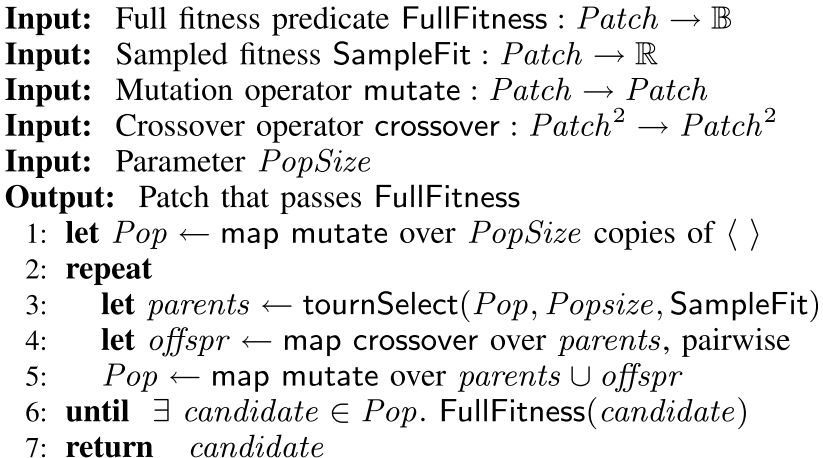
\includegraphics[width=\linewidth]{figs/gp.png}
\caption{Genetic Programming pseudocode.}
\label{fig:gp_pseudo}
\end{figure}

We believe this to be untrue and to verify our opinion we replace GP with NSGAII~\cite{nsgaii}. NSGAII is a incredibly popular variant of GA (18000+ citations). NSGAII consists of a novel sort algorithm that enables it identify better solutions and to converge at these solution much faster.  

\section{Methods and Materials}
\label{prelim}
Generally, when a bug is reported, an automated program repair tool based on a evolutionary algorithm undertakes a set of standard steps as endorsed by LeGoues et al~\cite{Goues}\footnote{Unfortunately, space limitations do not permit a detailed explanation of each of these steps, so this will brief.}.   

\begin{figure}[t]
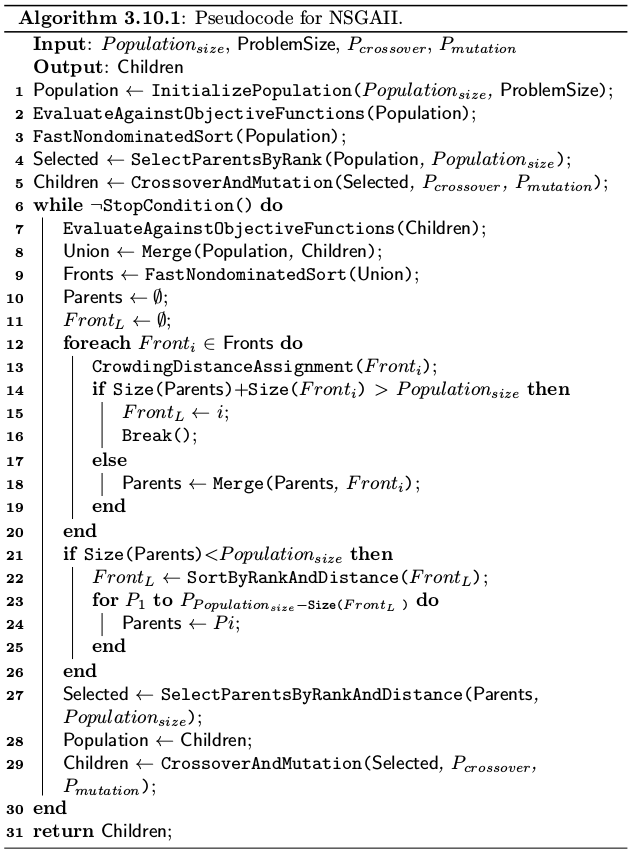
\includegraphics[width=\linewidth]{figs/nsgaii.png}
\caption{NSGA-II pseudocode. (Figure courtesy~\cite{clever})}
\label{fig:nsgaII}
\end{figure}
\subsection{Search Strategy}

GenProg proposes that use of an iterated stochastic search technique, to search for program repairs. Indeed, the search space comprising of possible repairs is extremely large, and any search algorithm would be required employ these four strategies to be a practical option: (1) generate coarse-grained, statement-level patches to reduce search space size; (2) implement fault localization to focus edit locations; (3) access existing code to provide the seed of new repairs; and (4) use a fitness approximation to cull bad patches.

In this paper, we discuss to such search strategies: GP and NSGA-II. Both of these are in fact variants of standard genetic algorithm. Motivated by studies on genetics, GA appeared in early 60s as a potential meta-heuristic search strategy. The rest of this subsection provides a very brief introduction to multiobjective search and the two algorithms\footnote{Interested readers are encouraged to read~\cite{clever} for a more in-depth discussion of these and other similar algorithms}.


\subsubsection{An Overview of Multiobjective Search}
\label{mos}
A multiobjective search is the task of finding solutions which satisfy two or more specified objectives. While a single-objective optimization involves a single objective function and a single solution, a multiobjective optimization considers several objectives simultaneously. 

In context of the current problem we have two potentially conflicting objectives: 
\be
\item Total number of failing test cases: needs to be minimized; and 
\item Number of test case executions before the first failure: needs to be maximized.
\ee

\begin{figure}[b]
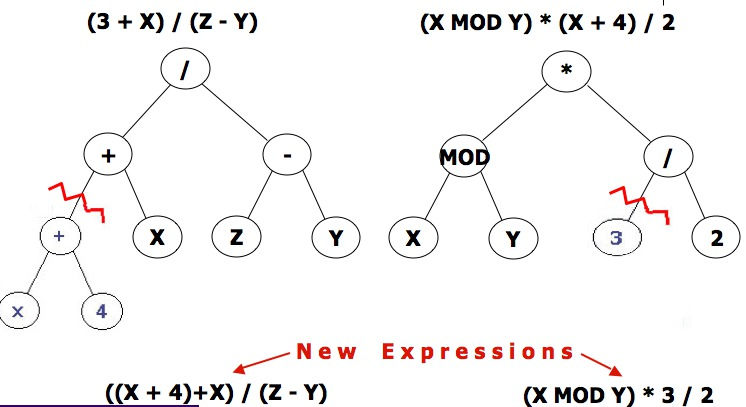
\includegraphics[width=\linewidth]{figs/gptree}
\caption{A contrived example of genetic programming on an AST.}
\label{fig:gp_ex}
\end{figure}

\begin{figure*}[tb!]
  \begin{minipage}{0.45\linewidth}
  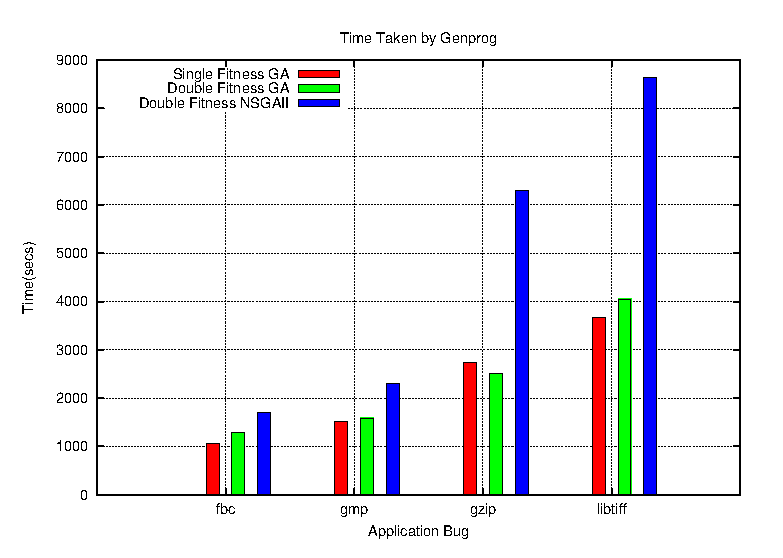
\includegraphics[width=\linewidth]{figs/time}
  \caption{Evalution Times of the search algorithms.}
  \label{fig:res_1}
  \end{minipage}~~~\begin{minipage}{0.45\linewidth}
  \centering
    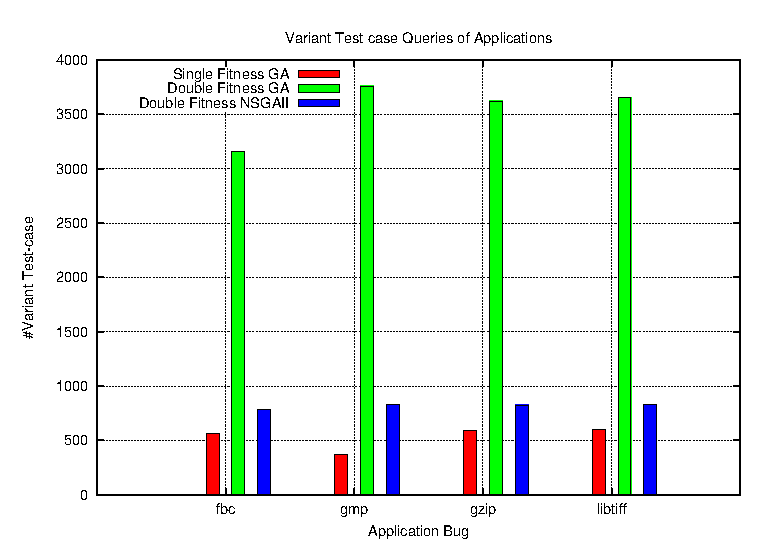
\includegraphics[width=\linewidth]{figs/variant}
    \caption{Exploration variance of the algorithms.}
    \label{fig:res_2}
  \end{minipage}
\end{figure*}
In such a case, a multiobjective optimizer generates a set of alternate solutions with certain trade-offs. These are called \textit{Pareto Optimal Solutions}. The solutions, in our case, will be a set of valid patches that perform equally well when measured in terms of the two objectives listed above.

Multiobjective problems are usually complex, NP-Hard, and resource intensive. Although exact methods can be used, they consume prohibitively large amounts of time and memory. An alternative approach would be to make use of meta-heuristic algorithms from RQ3. These approximate the Pareto frontier in a reasonable amount of time.

\subsubsection{Genetic Programming}

The Genetic Programming algorithm is inspired by population genetics (including heredity and gene frequencies), and evolution at the population level, as well as the Mendelian understanding of the structure (such as chromosomes, genes, alleles) and mechanisms (such as crossover and mutation). 

In the context of program repair, the objective of the Genetic Programming algorithm is to use induction to search potential patches. This is achieved by using evolutionary operators on candidate programs and their Abstract Syntax Trees to improve the adaptive fit between the population of candidate programs and an objective function. An assessment of a candidate solution involves the execution of given test cases counting the number of failures with a given patch.

High-level pseudocode for GenProg's main GP loop is shown in \fig{gp_pseudo}; it closely resembles~\cite{Goues}. Fitness is measured as a weighted average of the positive (i.e., initially passing, encoding required functionality) and negative (i.e., initially failing, encoding a defect) test cases. The goal is to produce a candidate patch that causes the original program to pass all test cases. In this paper, each individual, or variant, is represented as a repair patch stored and operated as an AST.  

\subsubsection{NSGA-II}

The objective of NSGA-II algorithm is to improve the adaptive fit of a population of candidate solutions to a Pareto front (see section~\ref{mos} for definition) constrained by a set of objective functions. The algorithm uses an evolutionary process with surrogates for evolutionary operators including selection, genetic crossover, and genetic mutation. The population is sorted into a hierarchy of sub-populations based on the ordering of Pareto dominance. Similarity between members of each sub-group is evaluated on the Pareto front, and the resulting groups and similarity measures are used to promote a diverse front of ``non-dominated'' solutions.


\fig{nsgaII} provides a pseudocode listing of the Non-dominated Sorting Genetic Algorithm II (NSGA-II) for minimizing a cost function. The \texttt{SortByRankAndDistance} function orders the population into a hierarchy of non-dominated Pareto fronts. The \texttt{CrowdingDistanceAssignment} calculates the average distance between members of each front on the front
itself.

\subsection{A Note on Patch Representation}
\label{patch_rep}
There are two fundamental differences between NSGA-II and GP. The first is of course, the nature of sort after each generation. NSGA-II uses a novel non-dominated sorting followed by an elite sampling to pick members that are retained in the population for the next iteration of the algorithm. GP on the other hand uses a simple \texttt{quicksort} followed by top-N sampling to pick members for the next iteration of the algorithm.

A more important distinction lies in the patch representation used by both these algorithms. NSGA-II converts the code in flattened representation. In a ``flat representation'' every line/expression is considered independent of every other line/expression. Mutations/Crossovers can affect any line. This is quite dangerous for obvious reasons. 

GP on the other hand takes a tree-based approach for code representation. It makes use of ASTs to represent the code. AST by nature respect code hierarchies and interdependencies. Thus, any mutation/crossover will not only affect a line, but will also affect the so-called children of that statement. A simple example is shown in ~\fig{gp_ex} for reference.


\subsection{Fault Localization}
After the search strategy is determined. An automated program repair scheme uses some form of fault localization to locate faults in a given code. GenProg\footnote{Note that when we say GenProg we refer to it as a scheme. All statements made about it apply to Genetic Programming and NSGA-II} focuses repair efforts on statements that are visited by the negative test cases, biased heavily towards those that are not also visited by positive test cases.
 
\subsection{Patch Generation}
Once faulty code snippet has been located, many candidate patches can be generated through the modifications to that code snippet, according to specific repair rules based on either evolutionary computation or code-based contracts. In the context of search, these would be solutions on the Pareto Frontier. Patches are represented as the source of insertion/replacement code pointed to on an AST (in the case of GP) or as line modifications to be performed (in case of NSGA-II). 

\subsection{Patch Validation}
When a candidate patch has been produced it is represented as a new AST (or new set of lines/expressions in the case of NSGA-II). The code is then modified to reflect these recommendations. This is followed by regression testing, inclusive of negative test cases (reproducing the fault) and positive test cases (characterizing the normal behaviors), is commonly used to validate the correctness of produced candidate patch. The above procedure can be iterated over and over again until some valid patch is found. Any patch passing all these test cases is considered valid. 

The fitness of a patch is a quantitative measure which is obtained by counting the following two measures: (1) Number of test case failure for a patch; and (2) Number of successful evaluations before the first test case failure. 

%\begin{figure}[!tb]
    \resizebox{1.01\linewidth}{!}{
		\begin{tabular}{ll}
			\hline
			\rowcolor[HTML]{EFEFEF} 
			\multicolumn{1}{l}{\cellcolor[HTML]{EFEFEF}{\bf Measure}} & \multicolumn{1}{c}{\cellcolor[HTML]{EFEFEF}{\bf  Description}}  \\ \hline
			\rowcolor[HTML]{FFFFFF} 
			{\bf Runtime}  & \begin{tabular}[l]{@{}l@{}}Time taken for the algorithm to be gener-\\ate optimal solutions.\end{tabular}\\\hline
			\rowcolor[HTML]{FFFFFF} 
			{\bf Speed Up}  & \begin{tabular}[l]{@{}l@{}}Ratio of time taken for the parallelized \\ version of the algorithm over the time\\taken for the serial version.\end{tabular}\\\hline
			\rowcolor[HTML]{FFFFFF} 
			{\bf Convergence}  & \begin{tabular}[l]{@{}l@{}}Convergence represents the accuracy of \\the obtained solutions. It is the distance\\between the obtained solutions and ideal\\Pareto frontier.\end{tabular}\\\hline
			\rowcolor[HTML]{FFFFFF} 
			\hline{\bf Diversity}                                           & \begin{tabular}[l]{@{}l@{}}Diversity represents the spread of the\\proposed solutions. Ideally the solutions\\should be well distributed across the Par-\\eto frontier,rather than concentrated in\\certain regions.\end{tabular}\\ \hline
		\end{tabular}}
		\caption{Performance Measures}
		\label{fig:measure}
	\end{figure}

\section{Evaluation}
\label{eval}
\subsubsection{Number of fixes}

This measure looks at the total number of bug fixes offered by the program. A successful program repair tool would at least generate one patch. A powerful tool should patch everything.  

\subsubsection{Evaluation Time}

As highlighted previously, multiobjective search algorithms are notorious for their impractically large run times. It is then important to measure how long a program takes to terminate. If the time taken is much larger than how much a human would take, it necessitates improving the algorithms or relaxing fitness criteria.

\subsubsection{Patch variance}

This measure is used to study the nature of patches generated by a search algorithm. It is entirely possible that a bug may be fixed in more that one way. Then, an method that can explore a much larger search space would be an enticing alternative to a narrow search scheme.  
\begin{figure}
  \begin{minipage}{\linewidth}
    \centering
    \begin{tabular}{l|l|l}
      Filename  & Lines & isFault \\ \hline
      dumpcap.c & 3           & 1.0     \\ \hline
      dumpcap.c & 123         & 1.0     \\ \hline
      dumpcap.c & 124         & 1.0     \\ \hline
      dumpcap.c & 1296        & 1.0     \\ \hline
      dumpcap.c & 2256        & 1.0     \\ \hline
      dumpcap.c & 2274        & 1.0    
    \end{tabular}
    \caption{Wireshark: Faults}
  \end{minipage} \\
  
  
    \begin{minipage}{\linewidth}
      \centering
      \begin{tabular}{l|l|l}
        Filename  & Lines & isFixed \\ \hline
        dumpcap.c & 3           & 1.0     \\ \hline
        dumpcap.c & 123         & 1.0     \\ \hline
        dumpcap.c & 124         & 1.0     \\ \hline
        dumpcap.c & 1296        & 1.0     \\ \hline
        dumpcap.c & 2256        & 1.0     \\ \hline
        dumpcap.c & 2274        & 1.0    
      \end{tabular}
      \caption{Wireshark: Patches}
    \end{minipage} \\
    
  \centering

\label{fig:fixedfiles}
\end{figure}

\section{Experimental Results}
\label{results}

\subsection*{RQ1: Can automated patch generation be modeled as a multiobjective search problem?}
To answer this question, we modeled GP as a two objective optimization and compared it with a single object GP that was available to us. The results we quite interesting, we found that a multiobjective GP fixed all the lines as the single objective GP. A sample \texttt{FaultFile} and \texttt{FixFile} are shown in Figure 6 and Figure 7. Note that in both the cases we obtained the exact same fixes in all the test programs. Thus, for parsimony's sake, we chose to report only one.

Therefore, this research question may be answered as follows:
\begin{lesson}
Yes. Automated patch generation \textbf{can} indeed be modeled as a multiobjective search problem.
\end{lesson}
 
\subsection*{RQ2: If yes, how does single objective GP compare to multiobjective GP?}
To answer this question, we study the evaluation time and test case variants. \fig{res_1} shows that in terms of runtime multiobjective GP is only slightly larger than traditional GP. But, more interestingly \fig{res_2} shows that multiobjective GP has a \textit{significantly  larger} variance than traditional GP. This is particularly interesting as it shows that multiobjective GP performs a more expansive search while looking for candidate patches.
  
Keeping these findings in view, this research question may be answered as follows.
\begin{lesson}
   Multiobjective GP is \textbf{significantly better} than simple GP in terms of patch variance. While also being \textbf{no worse} than simple GP in terms of evaluation times.
\end{lesson}

\subsection*{Can we replace genetic programming by some other genetic algorithm?}
To answer this question, we replaced GP with NSGA-II. We found, from ~\fig{res_1} and \fig{res_2}, that in addition to exorbitantly large runtimes in several cases, it fares no better in terms of variance. More importantly, NSGA-II fails to find any patch at all! Our findings are that this is due to a rather naive approach to patch representation used by NSGA-II, discussed in detail in \ref{patch_rep}.

Our findings lead to the following research answer:
\begin{lesson}
  Replacing GP with another genetic algorithm without a good patch representation approach is not advised.
\end{lesson}

\section{Discussions}
\label{discuss}

This report made an attempt to validate the efficacy of GP (as a multiobjective search) and the nature of mutate operations in GenProg. From RQ1 and RQ2 we note that, converting single objective GP to a multiobjective GP offers a significant benefits in that it performs a more expansive search for patches. From the outcome of RQ3 we find that GP owing to their tree-based mutation structure play a very important role in the operation of patch generation. Additionally, we found that NSGA-II failed to generate any patch, and this was due to the flattened representation of patches used by NSGA-II.     

\section{Future Work}
\label{conclusions}
In conclusion, our study introduced the use of multiple objectives in patch generation. It also show the importance of patch representation when performing a multiobjective search for patches.

As for future work, efforts must be taken to update the notation of patches prior to performing search. Also, other novel search strategies that use both GP and Non-dominated sort may be explored. In addition to this, the usefulness of a promising new algorithm called SWAY\footnote{This algorithm is in current development by our research group}~\cite{chen2016sampling, nair2016accidental} may be also be investigated.

\bibliographystyle{unsrt}
\bibliography{references}
\end{document}
